\documentclass[11pt,a4paper]{ivoa}
\input tthdefs
\input gitmeta

\usepackage{listings}
\lstloadlanguages{sh,make,[latex]tex}
\lstset{flexiblecolumns=true,numberstyle=\small,showstringspaces=False,
  identifierstyle=\texttt,defaultdialect=[latex]tex}

\usepackage{todonotes}

\usepackage[utf8]{inputenc}

\definecolor{texcolor}{rgb}{0.4,0.1,0.1}
\newcommand{\texword}[1]{\texttt{\color{texcolor} #1}}

\newcommand{\BibTeX}{Bib\TeX}

\iftth
 \newcommand{\comicstuff}[1]{
    \begin{html}<span class="comic">#1</span>\end{html}}
\else
  \newcommand{\comicstuff}[1]{(HTML exclusive material)}
\fi
\customcss{custom.css}

\title{The \ivoatex\ Document Preparation System}

\ivoagroup{Standards and Processes}

\author[http://www.ivoa.net/cgi-bin/twiki/bin/view/IVOA/MarkusDemleitner]{Markus Demleitner}
\author[http://www.ivoa.net/cgi-bin/twiki/bin/view/IVOA/MarkTaylor]{Mark Taylor}
\author[http://www.ivoa.net/cgi-bin/twiki/bin/view/IVOA/JamesDempsey]{James Dempsey}
\author[http://www.ivoa.net/cgi-bin/twiki/bin/view/IVOA/PatrickDowler]{Patrick Dowler}
\author[http://www.ivoa.net/cgi-bin/twiki/bin/view/IVOA/PaulHarrison]{Paul Harrison}
\author[http://www.ivoa.net/cgi-bin/twiki/bin/view/IVOA/MarcoMolinaro]{Marco Molinaro}

\editor{Markus Demleitner}

\previousversion[http://www.ivoa.net/documents/Notes/IVOATexDoc/20180814]{Version
1.2}
\previousversion[http://www.ivoa.net/documents/Notes/IVOATexDoc/20160430]{Version
1.1}
\previousversion[http://www.ivoa.net/documents/Notes/IVOATexDoc/20150129]{Version
1.0}
       

\begin{document}

\begin{abstract}
This note describes the \ivoatex\ document preparation system for IVOA
standards and notes.  \ivoatex\ supports the production of
PDF and HTML renderings of the documents with sources in
plain text suitable for version control, as is desirable for normative
texts.  This note contains a user guide as well as a discussion of 
\ivoatex's dependencies and its implementation.  It describes the
software as of May 2022 (release 1.2).
\ivoatex{} has special facilities for the git version control system,
and the default deployment uses github infrastructure.  Since at this
point github is the IVOA's designated version control system, this note
also contains material on the policies effective in the IVOA's use of
github.

\end{abstract}


\section*{Acknowledgments}

\ivoatex\ heavily draws from experiences made with previous markup-based
document preparation systems, in particular LaTeX classes and
infrastructure created by S\'ebastien Derriere and Mark Taylor, as well
as Paul Harrison's XML-based ivoadoc system.

We thank tth's author, Ian Hutchinson, for generous technical support
and prompt provision of solutions in the upstream source where necessary.

\section{Introduction}

Creating and developing standards is a  big part of the operations of
the International Virtual Observatory Alliance (IVOA).
As these are normative texts, attention to detail is very important, and
being able to rigorously track changes to the documents is highly
advantageous.  

Standards are also often developed cooperatively, which means that
capabilities for branching and merging are desirable.  This strongly
suggests employing version control systems for document authoring.
Change tracking in software designed for editing office documents, to
the extent it is supported at all, usually requires significant
manual intervention, is optional, often used incorrectly, and frequently
lacks interoperability.  Led by these considerations, it was decided that
\ivoatex\ would have to be based on plain text source files.

As mandated by the IVOA Document Standards \citep{2017ivoa.spec.0517G},
finished documents have to be at
least available in PDF, while an additional HTML rendering for online
use is recommended.  A document preparation system should thus be
able  to produce documents in these formats in at least acceptable
quality.

With these constraints in mind, several possible solutions were
investigated.  Paul
Harrison's ivoadoc
system\footnote{\url{https://volute.g-vo.org/svn/trunk/projects/ivoapub/ivoadoc}} 
went for XHTML as
an input format and used XSLT2 and XML-FO as document processors.  While
this facilitated several interesting features  -- for instance,
automatic extraction and formatting of XML schema fragments or
straightforward embedding of RDFa markup for machine-readable examples
--, it turned out that tooling issues were severe (e.g., reliable use
of SGML catalogs\footnote{This is important as retrieval of DTDs and
similar data from their commonly used system identifiers (i.e.,
typically W3C web servers) is at least undesirable and in practice
causes massive delays in formatting due to rate limiting on the part of
the W3C.}, non-free hyphenation patterns, classpath issues) and the use
of XML-FO for PDF generation yielded inferior renderings with little
prospect for improvements by third parties. Also, authors disliked
writing HTML tags.

Other options considered for source languages included docbook or 
a lightweight markup language (ReStructuredText and markdown having
been serious contenders).  
In each case, there were concerns either regarding the system's power
and flexibility or its ease of installation and maintenance.

Meanwhile, several documents -- to mention just a few, SAMP, VOTable,
and VOUnits -- had successfully used \TeX-based systems typically
derived from work done in the early 2000s by S\'ebastien Derriere.
\ivoatex\ essentially is a generalisation of these standards' formatting
systems, also inheriting from them the use of the \texttt{make} tool to
automate workflows.

\ivoatex\ was extended to relieve document editors from some of the
bookkeeping involved with producing IVOA standards and provide authors
with uniform solutions for common problems in standards typesetting.

In the remainder of this document, we give quick-start instructions
on installation and authoring in sect.~\ref{sect:quick} and continue
with
a more thorough discussion of \ivoatex's facilities, focusing
on enabling automatic production of both HTML and PDF output in
sect.~\ref{sect:authoring}.  Added in this document's version 1.3,
sect.~\ref{sect:ivoapol} then documents how ivoatex is intended to be
used on github by the various actors; authors and contributors to IVOA
standards should at least have a brief look at the recommended
procedures for them in subsection~\ref{sect:contributing}.
In sect.~\ref{sect:impl}, additional
details on the implemenation are given for the benefit of authors
planning to extend \ivoatex.  We close with a discussion of open issues
and desirable developments.

\section{Installation and Quick Start}
\label{sect:quick}

\subsection{Dependencies}

\ivoatex\ is designed to work more or less out of the box on common
POSIX-compliant systems; no non-free software is required for operation.
Its main uncommon dependency is the tth translator, 
a program based on lex used to translate LaTeX
to HTML.  As it is compact and portable, it is delivered with
\ivoatex~and built on demand.
Since \ivoatex's tth may at times offer
some enhancements over the upstream tth, using a system-installed tth is
discouraged.

The remaining dependencies include:

\begin{itemize}
\item A \LaTeX\ distribution with some commonly available packages (calc,
graphicx, xcolor, ifthen, doc, paralist, url, natbib, caption,
hyperref).
It is recommended to install TeXLive.
\item A sufficiently capable implementation of \texttt{make}, with GNU's
implementation recommended.
\item \texttt{librsvg2-bin} when people need to (re-) build architecture
diagrams.
\item Optionally, \texttt{latexmk}.  If it is available, a lot less
manual attention is necessary when rerunning LaTeX to update
bibliographies or document-internal references.
\item \texttt{python3} for  generated content and other housekeeping
that is probably not relevant for most authors.  Editors need it for
automatic submission to the document repository.
\item Editors will need the XSLT1 processor 
\texttt{xsltproc} (a different processor can
be used, but that would probably require custom make rules) for HTML
generation.
\item Editors will need the 
\texttt{gcc} compiler (another C compiler could be used; the
central makefile should probably be amended to allow easier changes
here), and \texttt{flex} for HTML generation.
\item Editors will need the \texttt{zip} archiver for package generation.
\item Editors will need \texttt{imageMagick} and \texttt{ghostscript} if 
vector graphics is to be processed into HTML.
\end{itemize}

Based on limited experience, we believe the easiest way to run
\ivoatex{} on Windows is through cygwin, which also should make make the
installation of the dependencies reasonably simple.

On
Debian-derived systems, the dependencies should be present after
running a distribution-specific adaption of
\begin{lstlisting}[basicstyle=\footnotesize]
apt install build-essential texlive-latex-extra zip xsltproc git\
  texlive-bibtex-extra imagemagick ghostscript cm-super librsvg2-bin
\end{lstlisting}
(cm-super contains vector versions of computer modern fonts in T1
encoding), on RPM-based systems something like
\begin{lstlisting}
yum install texlive-scheme-full libxslt make gcc zip\
  ImageMagick ghostscript git
\end{lstlisting}
should pull in everything that is necessary.

With OS X, a convenient way to obtain the dependencies is to install
MacPorts\footnote{\url{https://www.macports.org/}} and then run
\begin{lstlisting}
port install ImageMagick  libxslt ghostscript +full
\end{lstlisting}
The canonical OS\,X \TeX\ distribution is the Mac\TeX\ version of
\TeX Live\footnote{\url{https://www.tug.org/mactex/}}.  It is also
possible to build \TeX\ using MacPorts (with \texttt{port install
  texlive}), but this may result in a slightly non-standard
distribution.\footnote{See
  \url{http://tex.stackexchange.com/questions/97183/}.
  Also, MacPorts does add
  \texttt{texlive} as a dependency on many packages, and so frequently
  \emph{insists} on trying to build it; if you want to prevent this,
  there is some discussion at
  \url{http://comments.gmane.org/gmane.os.apple.macports.user/21526}.}

To see if the full prerequisites are there and compatible with \ivoatex, try
building an updated version of this document from its github source
(normal users can go without making HTML and packages, in which case a
lot of dependencies are not needed):
\begin{lstlisting}[basicstyle=\footnotesize]
git clone --recurse-submodules https://github.com/ivoa-std/ivoatexDoc
cd ivoatexDoc
make biblio   # update the bibliography
make forcetex # make a PDF ignoring timestamps
make ivoatexDoc.html  # make an html document
make package # make a zipfile for IVOA submission
\end{lstlisting}

During HTML generation, various diagnostics both 
from tth and from xsltproc (unknown commands,
unexpected end tags, and the like) are
expected at this point and no reason for alarm; we work on reducing the
amount of spurious error messages.

\subsection{Basic \ivoatex~operation}

For ease of installation and robustness, \ivoatex\ for now is designed
to be used from within a subdirectory of the directory containing the
document sources (rather than being installed globally).  Given that
it is fairly compact, having one copy per document seems acceptable.

So, the first step to use \ivoatex\ is to create a development
directory:

\begin{lstlisting}
export DOCNAME=SampleDoc
# this would be your document's short name, e.g., RegTAP, SIAv2)
mkdir $DOCNAME
\end{lstlisting}

The DOCNAME -- which will turn up in URLs, standard identifiers, and the
like -- should be chosen to be both succinct and expressive, and it
should not contain non-alphanumeric characters (the examples given here
assume that, too).  A name
like \texttt{SimpleDALRegExt} probably marks the upper limit in terms of
length.

While it is clearly preferable if authors use the IVOA's 
designated common version control system\footnote{Which, despite
many concerns \citep{book:zuboff}, currently is
github.com.} from the outset of
document development, it is possible to build ivoatex documents
locally as well.

\subsubsection{Installation from Archive (not recommended)}

Without version control, it is sufficient to obtain \ivoatex\ from a
distribution site and unpack it into the future document directory:

\begin{lstlisting}
cd $DOCNAME
curl http://ivoatex.g-vo.org/ivoatex-latest.tar.gz \
  | tar -xvzf -k
sh ivoatex/make-templates.sh $DOCNAME
\end{lstlisting}

The shell script will print some error messages because no version
control has been enabled.  These are safe to ignore.

\subsubsection{Installation with git version control}

The recommended way to run \ivoatex{}
is to use git's submodule feature.  This makes it very simple to keep
ivoatex up to date without polluting the
document's history, and it makes it straightforward to 
feed back any improvements you may make to ivoatex.  Hence, you will
usually start a document like this:

\begin{lstlisting}[basicstyle=\footnotesize]
cd $DOCNAME
git init
git submodule add https://github.com/ivoa-std/ivoatex
sh ivoatex/make-templates.sh $DOCNAME
git commit -m "Starting $DOCNAME"
\end{lstlisting}

The \verb|ivoatex/startup.sh| script will copy a few template files from
the ivoatex distribution to the working space.  You could do that
manually, too; see the script for what files to move where.

At this point, create a repository in your account using github.com's web
interface. Use \$DOCNAME as the repository name, and do not choose any
template; this procedure will leave you at a web page with a URI like
\nolinkurl{https://github.com/msdemlei/ivoatexDoc}.  
On that page, you can obtain a
``Clone URI'', which is what you can push to.  Use the ssh variant,
i.e., something like \verb|git@github.com:username/docname.git|.

Then, push your newly changed material into this new repository's main
branch:
\begin{lstlisting}[basicstyle=\footnotesize]
git remote add origin <Clone URI>
git push --set-upstream origin main
\end{lstlisting}
(depending on your git version and configuration, 
you may have to use ``master'' rather
than ``main'').

\subsubsection{Beginning the document}
\label{sect:beginning}

\paragraph{Main metadata in the Makefile}
\label{sect:mainmeta}

For convenience, the document production should start from some common
templates which are part of the \ivoatex\ distribution.  The above
procedure has already created \verb|README.md| (a brief introduction to
what the document is about), \verb|$DOCNAME.tex| (the future document)
and \verb|Makefile| (where some of the document metadata is defined).


The next step is to fill out the makefile template.  
As of the formatting of this document, this template looks like this:

\lstinputlisting[language=make,basicstyle=\footnotesize]{ivoatex/Makefile.template}

All lines with question marks must be filled out.  The document date
is the publication date, which can be significantly different from the
current date.  After its initial setting, it should only be changed at
the time of submission to the document archive.  It is always in
DALI-style ISO format \citep{2017ivoa.spec.0517D}, e.g., 2014-03-31.

\texttt{SOURCES} is used in dependency processing.  It would be amended
when the source file is split into separate files or if material is
included into the document, e.g., via \texword{lstinputlisting}.
Graphics files included do not need to be given here, as the document
will automatically depend on them.  The exception is
\verb|role_diagram.pdf|; see~sect.~\ref{sect:archdiag}.

\texttt{FIGURES} must contain the names of all bitmap graphics included
in the document; files missing here will be missing from the package for
distribution to the IVOA document repository, which will break the HTML
rendering.  As to \texttt{VECTORFIGURES}, see
sect.~\ref{sect:vectorgraphics}.

\texttt{AUX\_FILES} is intended for files that should be included in the
upload to the IVOA document repository while not taking part in the
actual formatting.  This in particular concerns XML Schema files, for
which the IVOA maintains a separate repository, but is by no means
limited to them. 

\ivoatex{} evaluates another variable, \verb|DOCREPO_BASEURL|, where you
can set a non-standard location of the formatted document.  This 
is only necessary for legacy documents, which is why the variable is not
mentioned in the template makefile.  For example, this document sets:
\begin{lstlisting}
DOCREPO_BASEURL=http://ivoa.net/documents/Notes/IVOATexDoc
\end{lstlisting}

\paragraph{Additional metadata in the \LaTeX~source}

The template for the \TeX\ source contains several lines with
multiple question marks.  These must be filled out as well.

As illustrated in the template, both \texword{author} and
\texword{previousversion} support an optional argument giving an URL; for
\texword{author}, it should normally point to the respective person's
page in the IVOA wiki, for \texword{previousversion}, it should point to
the landing page of the respective document version in the IVOA document
repository.  Further automation for maintaining document history
certainly is desirable, and the authors welcome ideas for how this might
look like.

\texword{ivoagroup} should contain the name of the (one) IVOA working or
interest group under which auspices the document development mainly
happens.  If this is an interest group (which is only possible for
notes), use \verb|ivoagroup[IG]{...}| to make \ivoatex~use ``Interest
Group'' rather than ``Working Group'' as the label of the corresponding
piece of metadata.

Pick one from the following list\footnote{We do not
enforce the use of the controlled vocabulary.  Automatic submission
with \texttt{make upload} will fail if you invent something here,
though.}:

\begin{compactitem}
\item Applications
\item DAL
\item Data Access Layer
\item Data Models
\item Grid and Web Services
\item Registry
\item Data Curation and Preservation
\item Standards and Processes
\item Semantics
\item Operations
\item Radio
\item Theory
\item VO Event
\item Time Domain
\item Education
\item No Group (only possible for Notes)
\end{compactitem}

\paragraph{The README}

The \verb|README.md| template should be edited to give a short
(one-paragraph) introduction to what the document is about at an even
higher level than the abstract.  The template also contains instructions
for building, pointers to the IVOA document repository, and a license
statement.  While you can change these if you want, that should not
usually be necessary.


\paragraph{The Architecture Diagram}
\label{sect:archdiag}

An architecture diagram is only 
necessary for documents on the recommendation track.  Notes may have
one, but since Notes are not shown on it, that is rather
unusual.  

To prepare an architecture diagram, first obtain the full description of
all IVOA standards:

\begin{lstlisting}
cp ivoatex/archdiag-full.xml role_diagram.xml 
git add role_diagram.xml
\end{lstlisting}

This is just an abstract specification that is compiled into images.  To
ensure this happens, \verb|role_diagram.svg| to \verb|FIGURES| in the
Makefile.  As long as the \LaTeX~toolchain does not support the SVG
image format, you must additionally append \verb|role_diagram.pdf| to
\verb|SOURCES|.

Then edit
\texttt{role\_diagram.xml} and remove all references to standards unrelated
to the current document.  As a rule, all \texttt{rec} elements for
standards not mentioned in
``Role within the IVOA Architecture'' should be removed.  Finally, use a
\xmlel{thisrec} element for the current standard.  An architecture
diagram for VOResource would thus be specified like this:

\begin{lstlisting}[basicstyle=\footnotesize]
<archdiag xmlns="http://ivoa.net/archdiag">
	<thisrec name="VOResource" x="64.5" y="155" w="71"/>
	<rec name="RegTAP" x="76" y="180" w="48"/>
	<rec name="Reg.Intf" x="75" y="205" w="50"/>
  <!-- and a few more -->
</archdiag>
\end{lstlisting}

The standard-specific
architecture diagram will be built by saying \texttt{make
role\_diagram.svg} and can be viewed using, for instance, common web
browsers.  Please refrain from editing the SVG with vector graphics
programs.  In the PDF renderings of the document, 
a PDF version of the architecture diagram is
required.  This is built using \texttt{make role\_diagram.pdf}, and a
stand-in will be built if your system lacks the software to do this
conversion (currently: rsvg-convert).

As long as the tooling situation regarding \LaTeX~and SVG is as
unsatisfactory as it is, please commit both \texttt{role\_diagram.svg} and
\texttt{role\_diagram.pdf} to the version control system.

\paragraph{Source code conventions}

\ivoatex\ requires the source to be written in UTF-8 encoding, since the
references shipped with it are in UTF-8.
Authors are urged to keep lines shorter than 72 characters in input
files whenever possible in order to keep diffs useful and readable.
When edits are made, paragraphs should not normally be reflowed to avoid
large diffs for minor edits.  Authors desiring a reflow after many edits
are encouraged to concentrate them in a separate, reflow-only commit.

\paragraph{Makefile targets}

The PDF version of the document is built by the makefile's default rule,
so running \texttt{make} will usually by enough.  This will produce a
file \texttt{\$DOCNAME.pdf}.

Other makefile targets for author use include:

\begin{itemize}
\item \texttt{biblio} updates the bibliography (i.e., runs \BibTeX);
running this is necessary after one of the bibliography files is updated
or when a new publication is referenced from the document.  This target
is not necessary on machines that have latexmk.
\item \texttt{forcetex} rebuilds the PDF unconditionally just as if the
main source had been edited.  This target is probably not useful on
machines with latexmk.
\item \texttt{\$DOCNAME.html} generates an HTML rendering of the
document; at this point, this will typically emit quite a bit of
spurious diagnostics.  Unfortunately, real problems may hide within.  
Therefore, we currently recommend a visual inspection of the resulting
HTML before submission.
\item \texttt{package} generates a zip file containing everything needed
for publication in the IVOA's document repository.   Obviously, 
\texttt{DOCVERSION}, \texttt{DOCTYPE}, and \texttt{DOCDATE} in the
Makefile should be updated as necessary before this target is built.
The result is a zip file with a name compliant to the IVOA document
standards \citep{2017ivoa.spec.0517G}.
\item \texttt{arxiv-upload}  produces a file arxiv-upload.tar.gz for
the current document.  ArXiv uploads are automatically done by the
document coordinator for RECs and ENs, and editors \emph{should not} do
them themselves.  Authors of Notes may upload their documents to arXiv.
\item \texttt{upload} produces a package, shows metadata to be uploaded to the
IVOA document repository (make sure everything is as you expect it) and
then uploads the package.
\item \texttt{generate} is used to update machine-generated content in
the document, typically by the main editor.  See
section~\ref{sect:generated} for details.
\item \texttt{update} updates the ivoatex submodule to whatever is in
the main ivoatex branch on github.  This will fail if you have
uncommitted local changes to your ivoatex.
\item \texttt{\$DOCNAME-draft.pdf} generates a PDF rendering just like a
simple make, but it will add a watermark against distribution.  This is
mainly intended for continuous integration workflows.  It only works
if \verb|pdftk| is installed.
\end{itemize}

\begin{admonition}{Note}
Simply running \texttt{latex}, \texttt{pdflatex}, 
or \texttt{mklatex} directly
(rather than through make) is \emph{not} supported with \ivoatex.  Due
to the non-global installation of the support files, the \TeX\ run needs
a special environment that is prepared by the makefile.

Also note that on systems without latexmk,
bibliography processing must be initated manually by
running \texttt{make biblio}; unless authors checked in the bbl file
this produces, this must be run after a document checkout.
\end{admonition}

\subsection{Examples}

Examples for \ivoatex\ use are found in the ivoa-std organisation on
github\footnote{\url{https://github.com/ivoa-std}}.


\section{Authoring documents}
\label{sect:authoring}

While \ivoatex\ documents can be written much like any other \TeX\
document, it is advisable to follow certain standards and use special
facilities for common appearance, easier development, and possible
evolution of \ivoatex\ itself.

\subsection{\ivoatex\ Features}

\ivoatex\ provides a small set of macros and environments designed
to ease standards authoring.  These include:

\begin{bigdescription}
\item[\texword{author}, \texword{previousversion}, \texword{ivoagroup}] these are discussed
in sect.~\ref{sect:beginning}.
\item[\texword{ucd}] a macro for marking up UCDs.  This in particular
helps with hyphenation of these, typically long, strings.
\item[\texword{xmlel}] a macro for marking up XML element or attribute
names and similar.  
\item[\texword{vorent}] for a name taken from VOResource or its
extensions, usually an
element or attribute name.
\item[\texword{admonition}] This is an environment for 
displayed boxes, intended for notes, tips, and the like.  
It takes an argument giving the head of the box, e.g.,

\begin{lstlisting}
\begin{admonition}{Note}
Admonitions should not be overdone.  
Also, they are floating insertions.
\end{admonition}
\end{lstlisting}
\item[\texword{bigdescription}] This is an environment for definition
lists in the style of HTML \xmlel{dl}, and it will be translated into
one.  Use \verb|\item[term]| for the term to be defined
(the construct this item is in is a \texword{bigdescription}).
\item[\texword{auxilaryurl}] A macro expanding a path relative to the
current document to a full URL.  This is discussed more extensively in
sect.~\ref{sect:links}
\item[\texword{inlinetable}] This is an environment for showing tables
in-place (rather than as an insertion potentially somewhere else, as
LaTeX's table environment does).  This may lead to rather empty pages
when the tables get longer.
\end{bigdescription}

The intention behind macros like \texword{xmlel} and \texword{vorent} is
that such terms are typeset uniformly across documents.  Further
semantic markup like this is planned for future releases, and document
authors are encouraged to contribute terms.

Also note that the title page is generated by the abstract environment.
Thus, all \ivoatex\ documents must have an abstract within the
\texword{abstract} environment.

\subsection{Listings, Verbatim Material}
\label{sect:verbatim}

\ivoatex\ documents should use the \texword{listings} package to include
source code snippets, XML fragments and the like.
Benefits over the \verb|verbatim| environment include easier control over
font size and formatting, the possibility to include external files,
and optional language-sensitive pretty-printing.
While the ivoa class
requires the package as of version 1.1 (and hence you can use the
\texword{lstlisting} environment without an explicit
\texword{usepackage} declaration), you will usually want to configure
the package in the document preamble (i.e., before its
\verb|\begin{document}|), perhaps like this:

\begin{lstlisting}
\lstloadlanguages{XML,sh}
\lstset{flexiblecolumns=true,tagstyle=\ttfamily,
  showstringspaces=False}
\end{lstlisting}

Additional
languages supported that are likely relevant in a VO context include C,
fortran, python, SQL, and java, specified as above case-insensitively.

The setup in the example (flexible columns, tags in
typewriter, no explicit blanks even in strings) 
produces reasonably pleasant output for a wide range of languages.

Actual listings are obtained with code like
\begin{verbatim}
\begin{lstlisting}[language=XML]
<example id="empty"/>
\end{lstlisting}
\end{verbatim}
Alternatively, entire files can be included like this:
\begin{verbatim}
\lstinputlisting[language=XSLT]{makeutypes.xslt}
\end{verbatim}
In the PDF rendering, the listings are pretty-printed
according to the value of the \verb|language| parameter if one is supplied.
This can aid comprehension, but in some cases the syntax-sensitive
processing can end up formatting the content in
unhelpful or distracting ways,
so authors should decide whether to supply a language value
or not, in which case output is simply \verb|monospaced|.
In the HTML rendering no pretty-printing is attempted in any case,
and the content is, currently, simply included in \xmlel{pre} elements.

If a more compact rendering of listings is desired, for instance,
because larger portions of source code are required in the document,
listings' \texword{basicstyle} option should be used together with one
of LaTeX standard size macros.  This could be in the argument of
\texword{lstset} in the preamble for a global setting, or on a
case-by-case basis as in

\lstinputlisting[language=tex]{verbatimstyles.tex}

As of version 1.2 of \ivoatex, only \texword{footnotesize} is actually
formatted by the CSS embedded in the HTML document, and we believe
listings should not be much smaller than that anyway.  As the options
are translated into CSS classes, it is fairly easy to add further
formatting functionality on a document-by-document basis, though.

\subsection{References and Bibliography}

\subsubsection{Built-in Bibliographies}
\ivoatex\ documents should use natbib and \BibTeX\ to manage references.
The package comes with two default bibliographies:

\begin{itemize}
\item \texttt{ivoatex/ivoabib.bib} containing records for many publications
likely to be cited by IVOA documents.  Feel free to add further records
if they might reasonably be cited by other IVOA documents.
\item\texttt{ivoatex/docrepo.bib} containing records for IVOA documents
listed in ADS, i.e., recommendations, endorsed notes, and a selection of
other notes.
\end{itemize}

Without latexmk, changes to the document that 
introduce new references or changes to the
bibliography require that \texttt{make biblio} is run before changes
become visible.

\ivoatex\ comes with a bibliography style of its own, derived from
\texttt{agsm.bst}.  The custom bibliography style was derived to
optimise some types of sources uncommon outside of the VO community, in
particular IVOA recommendations and notes.  Users are welcome to improve
\texttt{ivoatex/ivoa.bst}.

\subsubsection{Citation Style}

As usual in natbib, actual references are made through either writing
\verb|\citep{tag}|, yielding a form like ``(Einstein 1905)'',
or \verb|\citet{tag}|, yielding a form like ``Einstein (1905)''.
\ivoatex\ does not support variant forms of citep and citet (i.e., those
with optional arguments) yet; they will work in PDF output but fail in
HTML.  Contributions to improve this are welcome.

To reference an IVOA recommendation, locate its bibcode either using ADS
or directly within \texttt{ivoatex/docrepo.bib} and then use one of the
cite macros.  The preferred style is to introduce a short name for the
standard once with a citation and then use that short name in the
remainder of the document to have expressive texts not overciting. For
instance,

\begin{lstlisting}
IVOA Identifiers \citep{2016ivoa.spec.0523D} introduces URIs to
reference Registry records, which are typically transmitted in
VOResource \citep{2018ivoa.spec.0625P} format.  Both VOResource 
and IVOA Identifiers are based on various W3C standards.
\end{lstlisting}

will come out as

\begin{quotation}
IVOA Identifiers \citep{2016ivoa.spec.0523D} introduces URIs to
reference Registry records, which are typically transmitted in
VOResource \citep{2018ivoa.spec.0625P} format.  Both VOResource and IVOA
Identifiers are based on W3C standards.
\end{quotation}

Recommendations should generally be cited in the last version available
at the time of writing\footnote{If a published recommendation is missing
in the bibliography, this can be fixed by cd-ing into the ivoatex folder
and saying \texttt{make docrepo.bib}.}.  If works in progress (Working
Drafts, Proposed Recommendations) are to be cited, authors should create
a local bibliography (see below).

As part of bibliography management, authors should occasonally run

\begin{lstlisting}
make bib-suggestions
\end{lstlisting}

This will suggest updates to what IVOA standards the document cites
based on which documents obsoleted which other documents.  Note that
these suggestions should not be followed where references actually are
version-sharp.

\subsubsection{Local Bibliographies}

When a reference is really only relevant to a single document or is
conceptually non-permanent -- this, in particular, pertains to Working
Drafts or Proposed Recommendations to be cited --, it should be kept in a
local bibliography.  To instruct \LaTeX{} to use the references there,
the declaration at the foot of the document needs to be
changed to

\begin{lstlisting}
\bibliography{ivoatex/ivoabib,ivoatex/docrepo,localrefs}
\end{lstlisting}

Then a file \texttt{localrefs.bib} is created and checked into the
version control repository.  An example \BibTeX\ record for an
in-progress document is

\begin{lstlisting}
@Misc{wd:Datalink,
  author={Patrick Dowler and Francois Bonnarel and 
    Laurent Michel and Tom Donaldson and David Languignon},
  editor={Patrick Dowler},
  howpublished={{IVOA Working Draft 22 October 2013}},
  title={DataLink},
  year=2013,
  url={http://ivoa.net/documents/DataLink/20131022/}
}
\end{lstlisting}

Note that \emph{howpublished} contains the precise document date and the
\emph{url} points to the actual versioned landing page, not the generic
one for the standard.

\subsection{Graphics}

\subsubsection{Bitmap Graphics}

\ivoatex\ supports all bitmap graphics formats that pdflatex supports.
In practice, authors are encouraged to restrict themselves to JPEG, PNG,
and possibly GIF.  Currently, identical images are used for both PDF and
HTML renderings.  The recommended pattern for figures is
\begin{lstlisting}[language=tex]
\begin{figure}[th]
\begin{center}
\includegraphics[width=0.9\textwidth]{mydiagram.png}
\end{center}
\caption{A diagram of what this is about.}
\label{fig:mydiag}
\end{figure}
\end{lstlisting}
This gives \LaTeX\ some leeway in placing the figure, defines the image
size in units of the page width, and centres the image itself.

All bitmap graphics in a document must  be listed in the makefile's
\texttt{FIGURES} variable.  If they are not, the HTML rendering will be
broken.

\subsubsection{Vector Graphics}
\label{sect:vectorgraphics}

The only vector graphics format well supported in \ivoatex\ is PDF.  PDF
files can be directly used in \texword{includegraphics}.  The names of
such figures must be listed in the makefile's \texttt{VECTORFIGURES}
variable.

From \texttt{VECTORFIGURES}, \ivoatex\ arranges that, when a PDF figure 
\texttt{foo.pdf} is used, the HTML target depends on a file called
\texttt{foo.png}.  This PNG can be generated automatically by
\ivoatex\ using a combination of ghostscript and ImageMagick.  It may
sometimes be preferable to perform a custom conversion by hand (e.g.,
more compact representation with bilevel source images), in which case
the pre-rendered PNG should be included in the version controlled
repository.  This also
has the advantage that neither ghostscript nor ImageMagick are build
dependencies of the document.

\subsection{Tables}

In tables, rules should be used sparingly.  The standard pattern for tables is
something like
\begin{lstlisting}[language=tex]
\begin{table}[th]
\begin{tabular}{p{0.35\textwidth}p{0.64\textwidth}}
\sptablerule
\textbf{Column Head}&\textbf{Another column head}\\
\sptablerule
A value & Another value\\
A value in row 2& And so on\\
\sptablerule
\caption{A sample table}
\label{table:extable}
\end{tabular}
\end{table}
\end{lstlisting}

The \texword{sptablerule} used here inserts a horizontal rule with some
extra spacing and will be rendered consistently in both PDF and HTML.
It should not, as a rule, used between table rows. It is intended
primarily to delimit the table itself as well as the the heading and the
body.

\subsection{Hyperlinks}
\label{sect:links}

While \ivoatex\ puts no restrictions on the usage of hyperref features,
the preferred way to include links in \ivoatex\ documents is to use the
\texword{url} macro, i.e., use the URL itself as the anchor text.  In
this way, the link remains (to some extent) usable even if the document
is printed.  The alternative two-argument \texword{href} should
generally be avoided as it fails on paper.  For instance,
\begin{lstlisting}
(this is bad:) The \href{http://ivoa.net}{IVOA} has issued
\href{http://ivoa.net/documents}{many standards}.
\end{lstlisting}
would severely degrade when printed and is hence discouraged, whereas
\begin{lstlisting}
The IVOA\footnote{\url{http://ivoa.net}} has issued many 
standards, all of which can be retrieved from 
\url{http://ivoa.net/documents}.
\end{lstlisting}
works properly on all of \ivoatex's target media.

With non-HTTP URIs, it is recommended to use hyperref's
\texword{nolinkurl} macro (rather than an unadorned \texword{texttt} or
similar); advantages include that line breaking is better with
nolinkurl, less manual escaping is necessary, and, if desired, 
such URIs can be more easily styled.  An example:

\begin{lstlisting}
The value of the \xmlel{standardID} attribute will be
be \nolinkurl{ivo://ivoa.net/std/Registry#OAI-2.0}.
\end{lstlisting}

A special feature related to links is the \texword{auxiliaryurl} macro.
It is used when a document references a resource coming with the
document and versioned with it, but not included with the document text.
Examples for such material could be helper scripts, simple validators,
larger bits of sample data, and the like.  Note that vocabularies and
XML schema files should not be distributed in this way, as they have
conventional places within the ivoa.net URL hierarchy.

For instance, \verb|\auxiliaryurl{custom.css}| expands to
$$\hbox{\auxiliaryurl{custom.css},}$$ in this document, 
which is, for each release of this
document, the URL the example custom CSS file mentioned in the example
in sect.~\ref{sect:customcss} is found at.  The preferred way to include
such (long) URLs is in footnotes, as they typcially cannot be hyphenated.

In order to make \ivoatex~include the file linked to in this way in the
package submitted to the document repository, you must add the argument
of \texword{auxiliaryurl} to \verb|AUX_FILES| in the Makefile.

The macro needs to know where the document will be installed.  By
convention, this is \nolinkurl{https://www.ivoa.net/document/DOCNAME},
but historically, that convention was not always followed.  To make
ivoatex produce the correct URLs in those cases, use the
\verb|DOCREPO_BASEURL| makefile variable discussed in
sect.~\ref{sect:mainmeta}.

\subsection{Editorial tools}

When authoring standards, it is sometimes necessary to include
editorial comments of the type ``Need to clarify'' or ``Specification
incomplete''.  We recommend to use the todonotes package for such
pieces of text\footnote{Full documentation is available at
\url{http://www.tex.ac.uk/CTAN/macros/latex/contrib/todonotes/todonotes.pdf}.}.
It would be used like this:
\begin{lstlisting}
...
\usepackage{todonotes}
...
\begin{document}
\todo{This is an example for a editorial note}.
\end{lstlisting}

A rendering of such a to-do note is shown in this 
paragraph\todo{This is an example for a editorial note}. In HTML output,
only the simple \texword{todo} macro without options is supported, and
text is simply displayed inline right now.  Note in particular that
todonote's \texword{obeyDraft} and \texword{obeyFinal} package options
are ignored.  Although \ivoatex\ does not enforce it (yet), finished
recommendations should have no todo items in them.

While todonotes is a useful tool for standards development, we
discourage the use of packages to mark up changes, as maintaining such
markup usually is very hard, and version control offers a more
manageable solution to the problem such packages attempt to solve.

\subsection{Version Control System Information}
\label{sect:vcs}

It is recommended to include basic metadata obtained from the version
control system into \ivoatex~Documents where available.  
To enable in-document VCS metadata in git, two steps are necessary:

\begin{enumerate}
\item Add \texttt{gitmeta.tex} to your \texttt{SOURCES} in the makefile.
\item Add a line \verb|\input gitmeta| somewhere near the top of your
LaTeX source (right below \verb|\input tthdefs| is a good place).
\end{enumerate}

This will then add the commit identifier and a time stamp to the title
page of the document.  Patches to make ivoatex include some sensible URL
at which to look for a source repository might be found are welcome.


\subsection{Generated Content}
\label{sect:generated}

Sometimes it is desirable to have parts of a document generated through
some sort of ivoatex-external process.  Examples include copying
documentation from XML Schema files into the standard document 
or obtaining column metadata for standard
data models from a live TAP\_SCHEMA.

For such cases, \ivoatex\ offers a python script
\texttt{update\_generated.py}, which is executed by the
\texttt{generate} make target.  It simply looks for structured comments
in the main document and replaces what is between them with generated
contents.  The opening line consists of a \TeX~comment introducer, a
blank, the literal \texttt{GENERATED:}, another blank, and a command
line.  The closing line is a comment consisting of \texttt{/GENERATED}.

On running \texttt{make generate}, the material between the opening and
the closing line is replaced by the output of the command.

For instance, in the following snippet the material between the comments
was inserted by \texttt{make generate}:

\begin{lstlisting}
% GENERATED: echo This is generated content
This is generated content

% /GENERATED
\end{lstlisting}

\texttt{make generate} will not replace any content in the document source
if even just one command fails to execute as indicated by the
command's return code; it is transactional in this sense.

\ivoatex~will never execute \texttt{update\_generated.py} as part of a
dependency chain; it is intended that \texttt{make generate} must always
be manually triggered.  On the one hand, this is because its
dependencies cannot be generically modelled, given that arbitrary
commands can be executed.  Document authors are also discouraged from
providing such dependency information -- it is fairly common that
content generation depends on the availability of external resources
(e.g., databases or network services), and a document build should not
fail just because these are unavailable.

We mention in passing that generated content puts potentially executable
material into documents, which is of course an attack vector for
malicious software.  However, calling \texttt{make generate} is no
additional security risk, as whoever can change the document can
probably change the makefile, too, and the makefile can already contain
arbitrary commands that will be executed on the calling user's behalf.


\subsubsection{Built-in Generating Commands}

In addition to admitting arbitrary shell
commands, \texttt{update\_generated.py} has a facility that allows
calling special python functions from within documents: Commands
starting with an exclamation mark (``!'') are translated to calls to
appropriately named python functions defined within
\texttt{update\_generated.py}.

In the following, we document the built-in generating commands
(``builtins'') implemented in current ivoatex.

\paragraph{taptable}

The \texttt{taptable} builtin extracts documentation from a
live \texttt{TAP\_SCHEMA}.  The access URL of the
live TAP service must be specified in an environment variable TAPURL in
the Makefile, for instance

\begin{lstlisting}
TAPURL=http://dc.g-vo.org/tap
\end{lstlisting}

Then, in the document one can use the structured comment

\lstinputlisting[basicstyle=\ttfamily]{tapgen.tex}

After a \texttt{make generate}, the LaTeX source for a table describing
the columns of \texttt{tap\_schema.tables} will be between the two
comment lines; re-running \texttt{make generate} will replace that
content with a refreshed version.

\paragraph{schemadoc}

The \texttt{schemadoc} builtin formats
documentation for a type in an XML schema file.  This only works
properly if the XML schema defines a \xmlel{vm:targetPrefix} element in
the way pioneered by Ray Plante in
VOResource.\footnote{See
\url{https://github.com/ivoa-std/TAPRegExt} for a document using
schemadoc.}
With an appropriately instrumented schema, a document can say
\lstinputlisting{schemadoc-example.tex}
to produce documentation for the schema type \xmlel{MyType} within
the XML schema file \texttt{SchemaSource.xsd}.

\paragraph{vocterms}

The \texttt{vocterms} builtin formats the non-deprecated identifiers for
an IVOA vocabulary \citep{2021ivoa.spec.0525D} into a comma-separated
list.  It takes one argument, the vocabulary name (or, for legacy
vocabularies that have path-like names, the relative path; in practice:
whatever is behind \texttt{rdf/} in the vocabulary URI).  For instance,

\lstinputlisting[basicstyle=\ttfamily]{vocterms-example.tex}

will produce something like

\begin{quotation}
\noindent
% GENERATED: !vocterms datalink/core
\textsl{auxiliary},
\textsl{bias},
\textsl{calibration},
\textsl{coderived},
\textsl{counterpart},
\textsl{cutout},
\textsl{dark},
\textsl{derivation},
\textsl{detached-header},
\textsl{documentation},
\textsl{error},
\textsl{flat},
\textsl{noise},
\textsl{package},
\textsl{preview},
\textsl{preview-image},
\textsl{preview-plot},
\textsl{proc},
\textsl{progenitor},
\textsl{this},
\textsl{thumbnail},
\textsl{weight}
% /GENERATED
\end{quotation}

Note that vocabularies are designed to change over the lifetime of a
standard release.  Hence, whenever a standard gives such a 
list of identifiers, it should stress that that list is subject to
change and that clients should always fetch the current vocabulary from
the IVOA vocabulary repository.

\subsection{The Standards Record}
\label{sect:stdrec}

IVOA recommendations and endorsed notes must be registered using the
schema from StandardsRegExt \citep{2012ivoa.spec.0508H}.  A major use
case for this is to allow references to standards from other registry
records. The prototypcial example for this is the \xmlel{standardID}
attribute of VOResource \xmlel{capability} elements that contains
identifiers (and possibly standard keys as fragment identifiers)
declaring ``this service works as specified by that standard''.

Registration of IVOA-approved standards happens through the registry of
registries (RofR, authority ivoa.net).  The preparation of the registry
records, however, is up to the document editor.  It is strongly
recommended to keep and maintain the registry record in version control
alongside with the document source.

To do that, create a standards record from \ivoatex's template.  In a
clone of a repository using \ivoatex, you could say:

\begin{lstlisting}
$ cp ivoatex/stdrec-template.xml $DOCNAME.vor
$ git add $DOCNAME.vor
\end{lstlisting}

In the resulting file, the items one has to change are marked with four
hash marks; the elements \xmlel{schema} and \xmlel{key} can be removed
or repeated as required by a particular standard, all other elements
present should be given at least once.  Please remove the explanatory
comments as you go. 

This document comes with a filled-out sample for
itself\footnote{\auxiliaryurl{ivoatexDoc.vor}}.  This is
not to be uploaded into the Registry, as Notes are not (normally)
registered.

Most of the metadata to be filled in actually already is available in
structured form in \ivoatex.  Contributions that help automating
creation and maintenance of the standards record exploiting this are welcome.

With the upload of a proposed recommendation to the document repository,
the editor should send the standards record to the registry of
registries by e-mail\footnote{See \url{http://rofr.ivoa.net/} for
contact information.} and then re-submit the record with each upload or
a Recommendation or Endorsed Note; interim document states (WD, PR, PEN)
are not tracked by the Registry.


\subsection{Adding tests}

Many IVOA documents contain machine-readable artefacts or make
machine-verifiable claims.  If this is true for your document, consider
adding a \verb|test| target (since 2022, \ivoatex's template Makefile
alrady provides one).

The \verb|test| recipe should be designed so that

\begin{itemize}
\item the recipe fails if an assertion fails,
\item minimal (ideally no) output is produced for succeeding assertions,
\item extra (i.e., non-\ivoatex) software required to run the tests is
documented in a Makefile comment right above the recipe.
\end{itemize}

In the following, we discuss some typical scenarios for which tests
should be provided.

\subsubsection{Schema Validation}

Standards that come with XML schemas should validate both the schema and
one or more instance documents, which ideally should exercise as many
aspects of the schema as possible.  The instance files do not need to be
part of the released standard, although the auxilaryurl mechanism (see
sect.~\ref{sect:links}) would give a simple way to include these, too,
without overly impacting the document's appearance.

In order to limit the variety of tools editors may need, it is
recommended to use the \verb|xsdvalidate| subcommand of STILTS
\citep{2006ASPC..351..666T} for validation; this subcommand is available
only in STILTS versions 3.4-4 or later\footnote{The STILTS jar file can be
downloaded from \url{http://www.starlink.ac.uk/stilts/stilts.jar}}.
The VOResource
standard\footnote{\url{https://github.com/ivoa-std/VOResource}} shows an
example (edited here for clarity):

\begin{lstlisting}[basicstyle=\footnotesize]
STILTS ?= java -jar stilts.jar

# These tests need STILTS >=3.4-4
test:
  @$(STILTS) xsdvalidate VOResource-v1.1.xsd
  @$(STILTS) xsdvalidate \
    schemaloc='http://www.ivoa.net/xml/VOResource/v1.0=VOResource-v1.1.xsd' \
    example-voresource.xml
\end{lstlisting}

Some brief explanations are in order:

\begin{itemize}
\item Using a variable for STILTS allows one to easily override the
execution path if necessary (e.g., because of out-of-date system
packages or custom paths) like this:

\begin{lstlisting}
STILTS=stilts-beta make test
\end{lstlisting}

\item The comment specifies the dependencies to save later editors or
authors trial and error.  This becomes particularly important as test
suites grow.

\item The first line of the recipe validates the schema itself.  The
leading \verb|@| suppresses output, which reduces clutter in case
diagnostics are produced.

\item The second line of the recipe validates an instance document.  The
important thing here is to override the schema for the standard's target
namespace with the local copy of the schema; without the extra
\verb|schemaloc| parameter, STILTS would validate against the schema
from the document repository, which would both hide problems in the new
schema and lead to false positives in the instance document validated
(as it will not validate against the previous schema if it exercises new
features, which it should).  Further \verb|schemaloc| parameters,
pointing to either local files or network resources,
can be used if other schema locations need to be specified.
As in the example, use continuation lines (with backslashes)
to keep the command lines readable.

\end{itemize}

\subsubsection{Running Queries}

Where documents contain sample queries or requests, it is good practice
to automatically extract and execute these, ideally with some basic
checks for sane results.  An example for how this can be organised can
be found with the RegTAP
standard\footnote{\url{https://github.com/ivoa-std/RegTAP}}.  

To control the number of different tools editors might require, it
is recommended to base such code on either STILTS or pyVO
\citep{2014ascl.soft02004G}.

In RegTAP, which uses pyVO, the test rule looks like this 
(edited here for clarity):

\begin{lstlisting}[basicstyle=\footnotesize]
# These tests require python3 and pyvo (Debian: python3-pyvo)
test:
  @TAP_ACCESS_URL=http://dc.g-vo.org/tap python3 check_examples.py
\end{lstlisting}

The script \verb|check_examples.py| is too long to be reproduced in
full, but its core is:

\begin{lstlisting}[language=python,basicstyle=\footnotesize]
def main():
  svc = pyvo.dal.TAPService(TAP_ACCESS_URL)
  with open("RegTAP.tex") as f:
    for title, sample_query in iter_examples(f):
      try:
        result = svc.run_sync(sample_query).to_table()
        if not len(result):
          print(f"WARNING: Example returned no records in sect. '{title}'")
      except Exception as ex:
        print(f"ERROR: Example went bad in sect. {title}")
        print(ex)
        sys.exit(1)
\end{lstlisting}

Some notes on this:

\begin{itemize}
\item Again, suppress echoing of the commands make executes by prefixing recipe
lines with \verb|@| in order to keep the output tidy.

\item Tests of this kind will almost always use remote network
resources.  If possible, do not hide these within the (potentially
complex) Python code but make them explicit (and easily adaptable) in
the Makefile.

\item The Python fragment above should essentially do for any standard
discussing TAP queries. Note that the script distinguishes between
venial (empty results just give a warning and do not abort the
test run) and mortal (execution errors make the test run abort
immediately; the call to \verb|sys.exit| is important to make the entire
make rule fail) sins. It again will produce no output if everything runs
fine.

\item The \verb|iter_examples| generator used in the Python code is expected
to yield pairs of section titles and sample queries.  The code in RegTAP
uses heuristics strictly valid only for this document (e.g., queries in
lstlisting environments, subsections as the relevant sectioning
element).  The basic idea -- have some magic comment to signal that an
example is executable -- should be widely applicable, though.  
This way, a verifiable query in the instance document looks like
this:
\begin{lstlisting}[language=tex,basicstyle=\footnotesize]
%CHECK_HERE
\begin{lstlisting}[language=SQL,flexiblecolumns=true]
SELECT ivoid 
FROM rr.resource
...
\end{lstlisting}

\end{itemize}

\subsubsection{Miscellaneous Tests}

Tests can also come as simple shell commands (returning non-zero on
failure and emitting some diagnostics only in that case) as well.  Where
these go beyond one-liners, one should probably use a shell script.
Any dependency beyond the unix core tools should again be documented in
a Makefile comment right above the test rule.

An example for this type of check is again given in the VOResource
standard\footnote{\url{https://github.com/ivoa-std/VOResource}}, where
the test rule then would be:

\begin{lstlisting}[basicstyle=\footnotesize]
# These tests require xmlstarlet
test:
  @sh test-assertions.sh
\end{lstlisting}

The shell script called could run multiple tests, in particular if they
share some common infrastructure.  It is recommended to isolate each
test in a shell function with a name starting with ``assert'' and then
calling these shell functions as appopriate.  In the VOResource example,
where the authors make sure that if a Recommendation is being published,
the schema version tag actually is ``clean'', such a shell function
takes a shape like:

\begin{lstlisting}[basicstyle=\footnotesize]
assert_schema_version_for_rec() {
  # make sure the schema version has no tags if this is a REC
  if xmlstarlet sel -T -t -m "xs:schema" -v "@version"  $SCHEMA \
    | grep "^[0-9]\.[0-9]$" > /dev/null ; then
    : # all is fine, no output
  else
    die "$SCHEMA version has tags (inappropriate for a REC release)"
  fi
}
\end{lstlisting}

Note the STILTS package mentioned above includes some other tools
that may be useful for testing, for instance the subcommands
\verb|votlint| for checking VOTables and \verb|datalinklint| for
checking DataLink tables; see the
documentation\footnote{\url{http://www.starlink.ac.uk/stilts/sun256/cmdUsage.html}}
for details.
In particular it is a good idea to validate all example VOTable documents
included in document text.

\subsubsection{Testing Examples}

It is important to ensure correctness of literal example text appearing
in document content;
mistakes in examples confuse readers,
often get cut and pasted into operational systems,
and usually make it necessary to issue a document Erratum at a later date.

Mistakes in hand-written XML are particularly easy to make,
so providing Makefile tests for XML examples is strongly recommended.
This can be done by storing XML content in a file separate to the
document \LaTeX\ file and importing it with the \verb|\lstinputlisting|
macro as described in sect.~\ref{sect:verbatim}.
The XML file can then be tested (checked for well-formedness and,
where possible, validated) from a Makefile test target without reference
to the \LaTeX\ source.

If the included XML does not represent a complete document, it may be
necessary to use a container document that includes it using an
external entity reference defined in an internal DTD subset.
For example, suppose you want to include the following example text:
\lstinputlisting[basicstyle=\footnotesize]{fields.xml}
You can store that text in a file named \verb|fields.xml| and
include it in the \LaTeX\ source like:
\begin{lstlisting}[basicstyle=\footnotesize]
\lstinputlisting{fields.xml}
\end{lstlisting}
Then prepare a container document \verb|fields-container.xml| like:
\lstinputlisting[basicstyle=\footnotesize]{fields-container.xml}
and include a \verb|test| target in the Makefile like:
\begin{lstlisting}[basicstyle=\footnotesize]
# This test needs STILTS
test:
        $(STILTS) votlint votable=fields-container.xml
\end{lstlisting}


\subsection{Submitting a Document}

Snapshots of documents should be regularly submitted to the document
repository as part of the IVOA review process.  While \ivoatex~could
still make this a bit more streamlined, there is some automation for
this process present.  Consider the following recommendation for the
release process (of course, replace \verb|${DOCNAME}| with the DOCNAME
as defined in the Makefile):

\begin{enumerate}
\item Make sure your ivoatex is up to date; in git checkouts, run
\verb|make update| (or, equivalently, 
\verb|git submodule update --remote --rebase|).\footnote{\ivoatex{} before
July 2022 had a bug that would detach ivoatex's HEAD, which would
prevent \ivoatex{} updates from being pulled.  If unsure whether your
document is still affected, enter the \texttt{ivoatex} directory and run
% no \verb because we're in a TeX argument.
\texttt{git checkout master \&\& git pull} there.}

\item If the document contains generated content, run 
\verb|make generate| 
and inspect the subsequent output of 
\verb|git diff| 
for anything unexpected.

\item Add the version-specific URL and designation (e.g.,
``WD-20100801'') of the currently
published document (i.e., the version you are replacing) in the document
header using \texword{previousversion}.

\item Make sure the changelog appendix lists the major changes since the
last release of the document; it is probably a good idea to re-scan the
(generally more extensive) version control history at this point for
anything that is missing from the in-document changelog.

\item If you have schema files, vocabularies, or the like, make sure
their version identifiers are what you expect (in particular, for
recommendations, such version identifiers should have no appendices
of the kind ``-pr1'').  The \verb|AUX_FILES| variable in your Makefile is
a good start for what files to check.

\item For documents that provide a \verb|test| target, run 
\verb|make test|; 
this target must at least not error out and ideally not produce
any diagnostics.

\item Run \verb|make| and inspect \verb|${DOCNAME}.log|.  There should
obviously be no undefined citations or internal references.  Also, try
to avoid overfull hboxes (underfull hboxes are not always avoidable).

\item Have another round of proofreading on \verb|${DOCNAME}.pdf|.  Also
critically inspect the architecture diagram and the relationships to
other standards, in particular whether new versions of those have
reached REC in the meantime. \verb|make bib-suggestions| will do
that for you in the case of IVOA recommenations.

\item Run \verb|make ${DOCNAME}.html| and briefly review the produced
HTML file.  Warnings or even error messages in this process are
(regrettably) still to be expected, so at least superficial human inspection 
of the output is necessary.

\item Edit the Makefile and update the DOCVERSION, DOCDATE, and DOCTYPE
variables according to the new document release.

\item If uploading a REC or EN, update (or create) the standards record
and send it to the RofR (cf.~sect.~\ref{sect:stdrec}).

\item Run \verb|make package|.  If no major problems become visible,

\item run \verb|git commit -am "Preparing for the release"| (the message
should probably be more specific on \textit{which} release) -- this
will update the source if VCS information is represented as per
section~\ref{sect:vcs}.

\item Run \verb|make upload|.  This will ask you to review the document
metadata in a python dictionary, let you add a note for the document
coordinator and performs the upload.

\item Review the file \texttt{docrepo-response.html} created in the
document directory; this contains the raw HTML the uploading script got
back from the document repository.  We do not automatically check for
errors yet, so again human attention is required.

\end{enumerate}


\section{Developing IVOA Documents on Github}
\label{sect:ivoapol}

While \ivoatex\ can of course be used in private repositories, its
specific focus is the development of IVOA standards and related
documentation.  This section discusses practices and policies put in
place to ensure transparent and reproducible processes.  This is, by
necessity, closely tied to the IVOA's designated version control system,
github.


\subsection{The Organisations ivoa and ivoa-std}

As described above, documents will usually start in private
repositories.  At the latest when documents become become Proposed
Endorsed Notes or Working Drafts, they must move into the ivoa-std
organisation on github.  
Documents there are subject to certain policies ensuring
a controlled and well-documented evolution (cf.~sect.~\ref{sect:chmgt}).

For now, requests to move into ivoa-std are processed by the chair of
the TCG; they are usually filed by the chair of the working or interest
group handling the document.

For non-reviewed IVOA material, there is the github organisation ivoa.
Community members are welcome to use it for their VO-related projects
and in particular Notes.  However, there is no requirement to do that.


\subsection{Contributing to a Document}
\label{sect:contributing}

IVOA repositories for standards and notes on github follow many 
open source projects on that platform in using a fork 
and pull request workflow for contributing 
updates. This allows open contributions whilst protecting the repository
integrity. All contributors, whether document editors or first time 
contributors, follow this same process. All pull requests need to be 
approved by a maintainer of the repository.

When setting up your environment for a first time commit, we recommend
following the `triangle' workflow (Fig.~\ref{fig:triangleWorkflow}) to
make later contributions easier. 

\begin{figure}[th]
  \begin{center}
    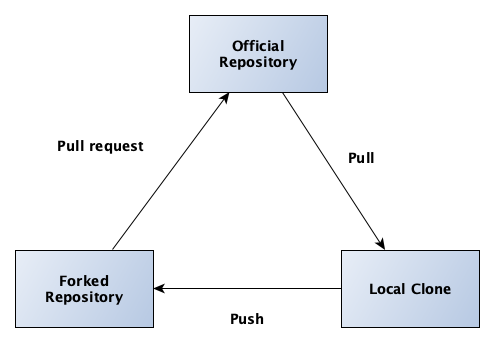
\includegraphics[width=0.9\textwidth]{triangle_workflow.png} 
  \end{center}
  \caption{The `triangle' workflow, where updates are made to a local
      copy of the official repository, pushed to a fork of the 
      repository and contributed back to the official repository 
      through pull requests.}
  \label{fig:triangleWorkflow}
\end{figure}

\begin{enumerate}

\item Fork the official repository using the `Fork' button on the upper
right of the repository's GitHub web page. This will create a copy of 
the repository under your user name which you can directly edit. See the
GitHub documentation 
\url{https://docs.github.com/en/get-started/quickstart/fork-a-repo} for 
further information.

\item On your local computer, clone the official repository and 
then add your fork as a remote repository. Note here that we use a 
read-only clone (https://) from the IVOA repository to avoid the potential
for future mistakes. 
\begin{lstlisting}[basicstyle=\footnotesize]
git clone  --recurse-submodules https://github.com/ivoa-std/standard.git
cd standard
git remote add mine git@github.com:username/standard.git
git remote -v
\end{lstlisting}

you should see output similar to 
\begin{lstlisting}[basicstyle=\footnotesize]
mine  git@github.com:username/standard.git (fetch)
mine  git@github.com:username/standard.git (push)
origin  git://github.com/ivoa-std/standard.git (fetch)
origin  git://github.com/ivoa-std/standard.git (push)
\end{lstlisting}


\item Now to prepare for your change, make sure you are up to date with
the official repository and create a branch for your work.
\begin{lstlisting}
git checkout main
git pull origin main
git checkout -b branch-name-for-change
\end{lstlisting}

IVOA repositories are transitioning from using ``master'' as the main
branch to using ``main''.  Depending on the repository, you may need to
adapt the above commandline accordingly.

\item Once you are happy with the change (and we do recommend building
the PDF document locally to review it) you can save it to git and send 
it to your forked repository.  The status command will list everything 
that has changed and the add command will include it the commit.

\begin{lstlisting}
git status
git add standard.tex another-changed-file
git commit  -m "a  short and useful description of my changes"
git push mine branch-name-for-change
\end{lstlisting}

\item  Then, on the GitHub web interface for your repository, create
your Pull Request to contribute it back to the official repository.

\item  Wait for reviews, update the change as needed, repeating step 4
for each set of changes. Once the change is approved by a maintainer,
the maintainer may merge your change themselves or leave you to merge
once you are ready.
\end{enumerate}

For future changes repeat steps 3 to 6.

\subsection{Enabling Continuous Integration}

\ivoatex{} can set up continuous integration workflows that
automatically build documents on github infrastructure.  Editors can
enable these workflows by running the following commands in the document
directory:

\begin{lstlisting}
make github-preview
git commit -m 'Add/Update gh-Workflows for PDF Preview'
git push
\end{lstlisting}

This arranges for a document build to be run at every change to the main
branch and when a pull request is created.  Since the github's workflow
engine will spin up a container for that and install \ivoatex's
prerequisites on that, this may take of order of minutes.  For a pull
request, the built PDF is found under the ``Checks'' tab and then in
``Artifacts''.

After merges into the main branch, the built PDF becomes available under
Releases $\to$ Auto PDF Preview.  You may want to have a link toward
this PDF preview; in that case, simply include the Markdown snippet that
the above make command prints into \verb|README.md|.


\subsection{Managing Changes}
\label{sect:chmgt}

This section should be read by persons serving as document editors.

The role of a document editor is to ensure that a document eventually
converges towards a cohesive text, where an editor may or may not be one
of the document authors.  Editors should also make sure that
document changes are always well-documented and open to later scrutiny.
The goal should be that later readers can find out why a given change
was made, i.e., what new functionality it was intended to provide or
what problem it should address.

While a document is under public review, the editor's role as the text's
gatekeeper is particularly important.  In particular, they must ensure
that all changes are properly reviewed and do not introduce changes so
profound that a new full review would be required.

With these considerations, the following policies apply to documents
under IVOA management:

\begin{enumerate}
\renewcommand\theenumi{\alph{enumi}}
\item Nobody can commit directly to the main branch of a document.
Instead, all changes go through pull requests, where editors take care
that titles and descriptions are suffiently clear and complete.

\item Before public review (i.e., in the state of a Note, a Working
Draft, or a Proposed Endorsed Note before TCG review), it is at the
editor's discretion whether they want individual pull requests reviewed
separately or whether pull requests are merged without a further review.
To give some examples, a pull request adding a major feature could be
announced on the pertinent IVOA mailing list and undergo some sort of
public pre-review, whereas a re-working of a section could profit from a
formal review by a co-author.  A pull request just repairing some
bibliographic references can be merged by the editor directly.

\item For documents under public review (i.e., Proposed Recommendations
and PENs under TCG review), all pull requests must be reviewed, where at
least one reviewer should be a document author.  It is the editor's duty
to find reviewers, where obviously the persons who brought up the points
addressed by the pull request would be particularly good choices.
\end{enumerate}

In order to ensure document histories remain readable, editors are
encouraged to squash-merge pull requests that only contain closely
related commits.

\subsection{Adopting a Repository for ivoa-std}

This section documents policies and workflows for the managers of the
ivoa-std organisation; normal \ivoatex~users can ignore it.

On request by a chair of an IVOA working group, the ivoa-std management
will migrate a repository from where the original editor started it
(called \verb|<original-repo>| below) to the ivoa-std organisation.  To
do that, they perform the following steps:

\begin{enumerate}
\item Inspect the \verb|<original-repo>| and make sure it includes the minimal
files: README.md, LICENSE, Makefile, ivoatex submodule, and a LaTeX
file with the proposed \verb|<short-name>|
\item Create a new public repository \verb|ivoa-std/<short-name>| via github's
browser UI and using the ``import'' facility to import the
original repository
\item Make a local clone and build the document; if this fails, create an issue
for the original author(s) to fix before any work can proceed
\item Optional: add github workflow, commit, and push directly to main branch
\item Setup branch protection rules for the main branch (see below)
\item Give the WG team and the editor admin privileges (see below)
\item Notify the WG and the editor of the move via the WG's mailing list
\item Notify the original owner, noting that \verb|<original-repo>|
should be renamed and preserved for a while, while the repository must
now be forked from ivoa-std in order to enable future pull requests
(cf.~sect.~\ref{sect:contributing})
\end{enumerate}

Branch protection rules are set up in the ``Settings'' tab of the repository (top right). 
On the left side of the settings page, choose ``Branches'' and either edit the \verb|main|
branch rules (if present) or add a new rule (if not). The standard set of rules that are
suitable for most development are:

\begin{enumerate}
\item Require a pull request before merging
\item Require approvals
\item Dismiss stale pull request approvals when new commits are pushed
\item Require status checks to pass before merging (see below)
\item Require branches to be up to date before merging
\end{enumerate}

The status checks requirement can be enabled before an actual check (github workflow) is
added or found by the system. Repository administrators may have to come back and enable a 
specific status check workflow after it is added (behaviour is a little opaque here).

By not enabling ``Include administrators'', repository admins will be able to override the 
approval requirement and merge pull requests that do not require review (e.g., fixing the build,
updating Makefile settings, etc).

Granting admin privileges to the WG (there is a team setup for each WG) is also done in the 
``Settings'' tab. On the left side of the settings page, chose ``Collaborators and teams''
and then ``Add teams'' (green button on the right). Start typing the WG name or acronym (e.g.
dal or reg) and then select the complete group name from the popup. The WG teams are all
of the form \verb|ivoa-std/<group>-admin|; the complete list can be found from the top-level 
\verb|ivoa-std| organization page in the ``Teams'' tab.

\section{Customisation and Development}
\label{sect:impl}

This section discusses aspects of \ivoatex\ that are more technical in
nature.  Authors with a modicum of \TeX\ expertise are nevertheless
encouraged to read it.

\subsection{Technical Overview}

The central files in \ivoatex\ processing are

\begin{bigdescription}
\item[ivoa.cls] The class file, inheriting from \LaTeX's article class.
The file defines the markup rules for PDF processing, including
titlepage generation and extra macros and environments.  Its content is
ignored for HTML generation.

\item[tthdefs.tex] This file protects its contents from normal \TeX\
processing by a \verb|\iftth| conditional. This way, only tth sees
definitions made here. Each special feature defined in \texttt{ivoa.cls}
has a counterpart here, giving rules for its translation to HTML.  This
usually encompasses emitting some HTML before and after the argument of
a TeX construct, where material between \verb|\begin{html}| and
\verb|\end{html}| is included literally in the HTML document.

\item[tth-ivoa.xslt] An XSLT stylesheet that postprocesses tth's output
and performs some operations that would be inconvenient to implement in
\texttt{tthdefs.tex}, in particular for the formatting of the opening
material.

\item[Makefile] This makefile is included by the user makefile in the
document directory proper.  It defines the rules given above as well as
some extra housekeeping rules like package building and building tth
from its source.

\end{bigdescription}

\subsection{Semantic Markup}

In order to make it support rich, semantic markup, \ivoatex\ needs to be
continuously developed.  In particular, it is good practice to define
macros for marking up values of certain datatypes, as with \ivoatex's
\texword{xmlel} and \texword{vorent}.  
Thus, whenever a document has multiple
instances of such values, authors should define macros and use these.
For instance, RegTAP deals with lots of concepts from its own
database schema and hence has
\begin{lstlisting}
\definecolor{rtcolor}{rgb}{0.15,0.4,0.3}
\newcommand{\rtent}[1]{\texttt{\color{rtcolor} #1}}
\end{lstlisting}
in its document preamble to
define markup for ``RegTAP entity'', whereas
this note, as it mentions many words with a special meaning to \TeX, has
\begin{lstlisting}
\definecolor{texcolor}{rgb}{0.4,0.1,0.1}
\newcommand{\texword}[1]{\texttt{\color{texcolor} #1}}
\end{lstlisting}
Such macros will be included in \ivoatex\ itself rather than an
individual document's preamble when they prove useful in multiple
documents.

\subsection{Custom Macros and Environments}

The tth translator used by \ivoatex\ ignores \texword{usepackage}.  Many
common packages are natively supported, but those that are not in
general need specific handling, and sometimes support is somewhat spotty.  
For instance, the \texword{nolinkurl}
macro is not supported natively by tth, and hence in
\texttt{tthdefs.tex} there is code to the effect of
\begin{lstlisting}[basicstyle=\footnotesize]
\def\nolinkurl#1{\special{html:<span class="nolinkurl">}%
  \verb|#1|%
  \special{html:</span>}}
\end{lstlisting}

When a document requires special markup, it is likely that 
different implementations will be necessary for PDF and HTML output.
Using \texword{iftth} the implementations for the current output mode
can be selected (without the \texword{newif} mentioned in the tth
documentation, as that is already performed in \texttt{tthdefs.tex}).

For instance, RegTAP 1.0 had many inline tables that need special spacing
for the PDF rendering, whereas normal tables will do for them
in HTML.  It therefore
had in its preamble the definitions
\begin{lstlisting}
\iftth
  \newenvironment{inlinetable}{}{}
\else
  \newenvironment{inlinetable}{\vskip 1ex\vfil
    \penalty8000\vfilneg%
    \hbox to\hsize\bgroup\hss}
  {\hss\egroup\vspace{8pt}}
\fi
\end{lstlisting}

(this mechanism proved useful for other specifications, too, and so
it is part of \ivoatex~proper now).

\subsection{Custom CSS}
\label{sect:customcss}

If you find you need custom CSS to fix HTML formatting, you should
probably talk to \ivoatex's authors first.  There are, however, 
legitimate cases when something needs extra styling in HTML that 
comes out right without further effort
in the PDF output.  In such cases, a custom CSS file can
be added to a repository (it must then also be added to \texttt{SOURCES}
in the Makefile in order for it to be delivered with the document
package).

The document itself would then use the \ivoatex's \texword{customcss}
macro in its preamble with the CSS file name as an argument.  For
example, the source for this document says

\begin{lstlisting}
\iftth
 \newcommand{\comicstuff}[1]{
    \begin{html}<span class="comic">#1</span>\end{html}}
\else
  \newcommand{\comicstuff}[1]{(HTML exclusive material)}
\fi
\end{lstlisting}

\noindent in its preamble.  With this and a CSS
file\footnote{\auxiliaryurl{custom.css}},

\begin{lstlisting}
\comicstuff{If this is comic sans, your web browser is permissive.}
\end{lstlisting}

\noindent becomes: 
\comicstuff{If this is comic sans, your web browser is permissive.}

\subsection{Maintenance of the Architecture Diagram}

The IVOA architecture diagram is used by
\citet{2021ivoa.spec.1101D} to
visualise the standards landscape.  All IVOA recommendations should have
an architecture diagram showing the current standard as well as the
related standards within that landscape.

Within \ivoatex, architecture diagrams are produced in Scalable Vector
Graphics (SVG).  The source is in \texttt{ivoatex/archdiag-full.xml},
specifying the location of the recommendations (in \xmlel{rec} elements)
and the documents on the recommendation track (in \xmlel{prerec}
elements).  The figure has a design size of $800\times 600$ ``pixels''.
Note that SVG is not really pixel-based -- the numbers are just
convenient, unitless floating point numbers, and the conversion of these
coordinates to physical ones is done at render time.

In the diagram, the standards shoud be limited to the inner box, i.e.,
the zone between 50, 100 and 750, 500.  Standards boxes are 
18 pixels high, which is set in the \texttt{format-standard} template
in \texttt{make-archdiag.xslt}.  Their widths default to 90 pixels, but
when you add a box in \verb|archdiag-full.xml|, please take a moment to
provide a \verb|w| attribute.  See the opening comment of
\verb|archdiag-full.xml| for a brief howto on having the machine compute
it.

When standard boxes are aligned, the
vertical distance of their centres should be 25 pixels, the horizontal
distance 100 pixels.  To keep the diagram lively, standards not
obviously grouped with others may be placed ``off-grid''.

The specifications in \verb|archdiag-full.xml|, as well as those in
the authors' \verb|role_diagram.xml|, are ad-hoc XML interpreted by the
stylesheet \verb|ivoatex/make-archdiag.xml|.  That stylesheet is
written such that all three levels of the architecture diagram can be
created.  The \verb|Makefile| in \verb|ivoatex| has the necessary
rules, but in contrast to the author rules, they are expected to be
executed \emph{within} the ivoatex directory.

So, to create the full versions of the three levels of the architecture
diagram, do something like

\begin{lstlisting}
cd ivoatex
make archdiag-l0.svg
make archdiag-l1.svg
make archdiag-l2.svg
\end{lstlisting}

The resulting svg files can be viewed in common browsers or in vector
graphics programs like inkscape.  The latter can also be used to find
good positions for new elements (cursor coordinates are shown in the
footline, but the direction of the y axis is reversed versus the SVG
coordinates).  Please do not use graphical tools to edit the diagram
itself -- the goal of the current architecture is to make edits
transparent and have a clear and simple specification of the standards
themselves in a file producing meaningful diffs.

\section{Desirable Features to be Implemented}

A major drawback of \ivoatex's HTML output is that paragraphs are not actually
marked up as such.  Due to the \TeX\ processing model, their
reconstruction is non-trivial.  Hence in the generated HTML,
source-level paragraphs are rendered as text nodes separated by empty
HTML paragraph elements.  It would probably be possible to rectify this
in the XSLT postprocessing.

An automated way to maintain the in-document history (i.e., the sequence
of \verb|\previousversions| in the preamble) and better support to
generate the change log would be desirable.

The biblio and forcetex targets behave in somewhat confusing ways.
Perhaps we should simply make latexmk a hard dependency and forget about
them?

\appendix
\section{Changes from Previous Versions}

\subsection{Changes from Version 1.2}

\begin{itemize}
\item Changed instructions to use github rather than volute.
\item Added a best practice on contributing via github.
\item Added policy sections for editors and the IVOA github maintainer.
\item Added info on a few new ivoatexDoc features (e.g., the ucd macro).
\item Added a section on writing regression tests.
\item Now mentioning bib-suggestions for bibliography maintenance.
\item Expanded the submission checklist.
\item Dropped a section on ivoadoc migration; it's unlikely anyone
will need that any more.
\end{itemize}

\subsection{Changes from Version 1.1}

\begin{itemize}
\item Added material on the SVG architecture diagram, removed references
to old PNG-based workflow.
\item Added an upload checklist (and, relatedly, listing legal WG names).
\item Added documentation on auxiliaryurl.
\item Added instructions on making standards records.
\item Documented triple-bibliography maintenance.
\end{itemize}

\subsection{Changes from Version 1.0}
\begin{itemize}
\item Changed google code URLs to volute.g-vo.org ones.
\item Documented new facilities for generating material, with extra
focus on auto-documenting XML schema.
\item Added advice on citing IVOA recommendations.
\item Re-targeting for \ivoatex 1.0 (rather than 0.4 before)
\end{itemize}


\bibliography{local,ivoatex/ivoabib,ivoatex/docrepo}


\end{document}
